\subsection{Reeb and Mapper graphs}
\label{subsec:reeb_mapper_def}

%\subsubsection{Reeb graphs}
We start by introducing Reeb graphs defined on general topological spaces.
\begin{definition}{Reeb graph.}\\
    Let $\spa$ be a topological space and let $f\,:\,\spa\rightarrow \R$ be a continuous %(sometimes Morse-type) 
function called {\it filter function}. Let $\sim_{f}$ be the equivalence relation between two elements $x$ and $y$ in $\spa$ defined by: $x\sim_{f} y$ if and only if $x$ and $y$ are in the same connected component of $\preim{f}{\{v\}}$ for some $v$ in $f(X)$. 
%We then define the Reeb graph as:
 The Reeb graph $\Reeb_f(\spa)$ of  $\spa$ %computed with a filter function $f$ 
is then defined as the quotient space $\spa/\sim_{f}$.
\end{definition}

Figure \ref{fig:reeb_graph_example} provides an illustration of a Reeb graph computed on a torus with its height as filter function.

\begin{figure}[t]
    \centering
    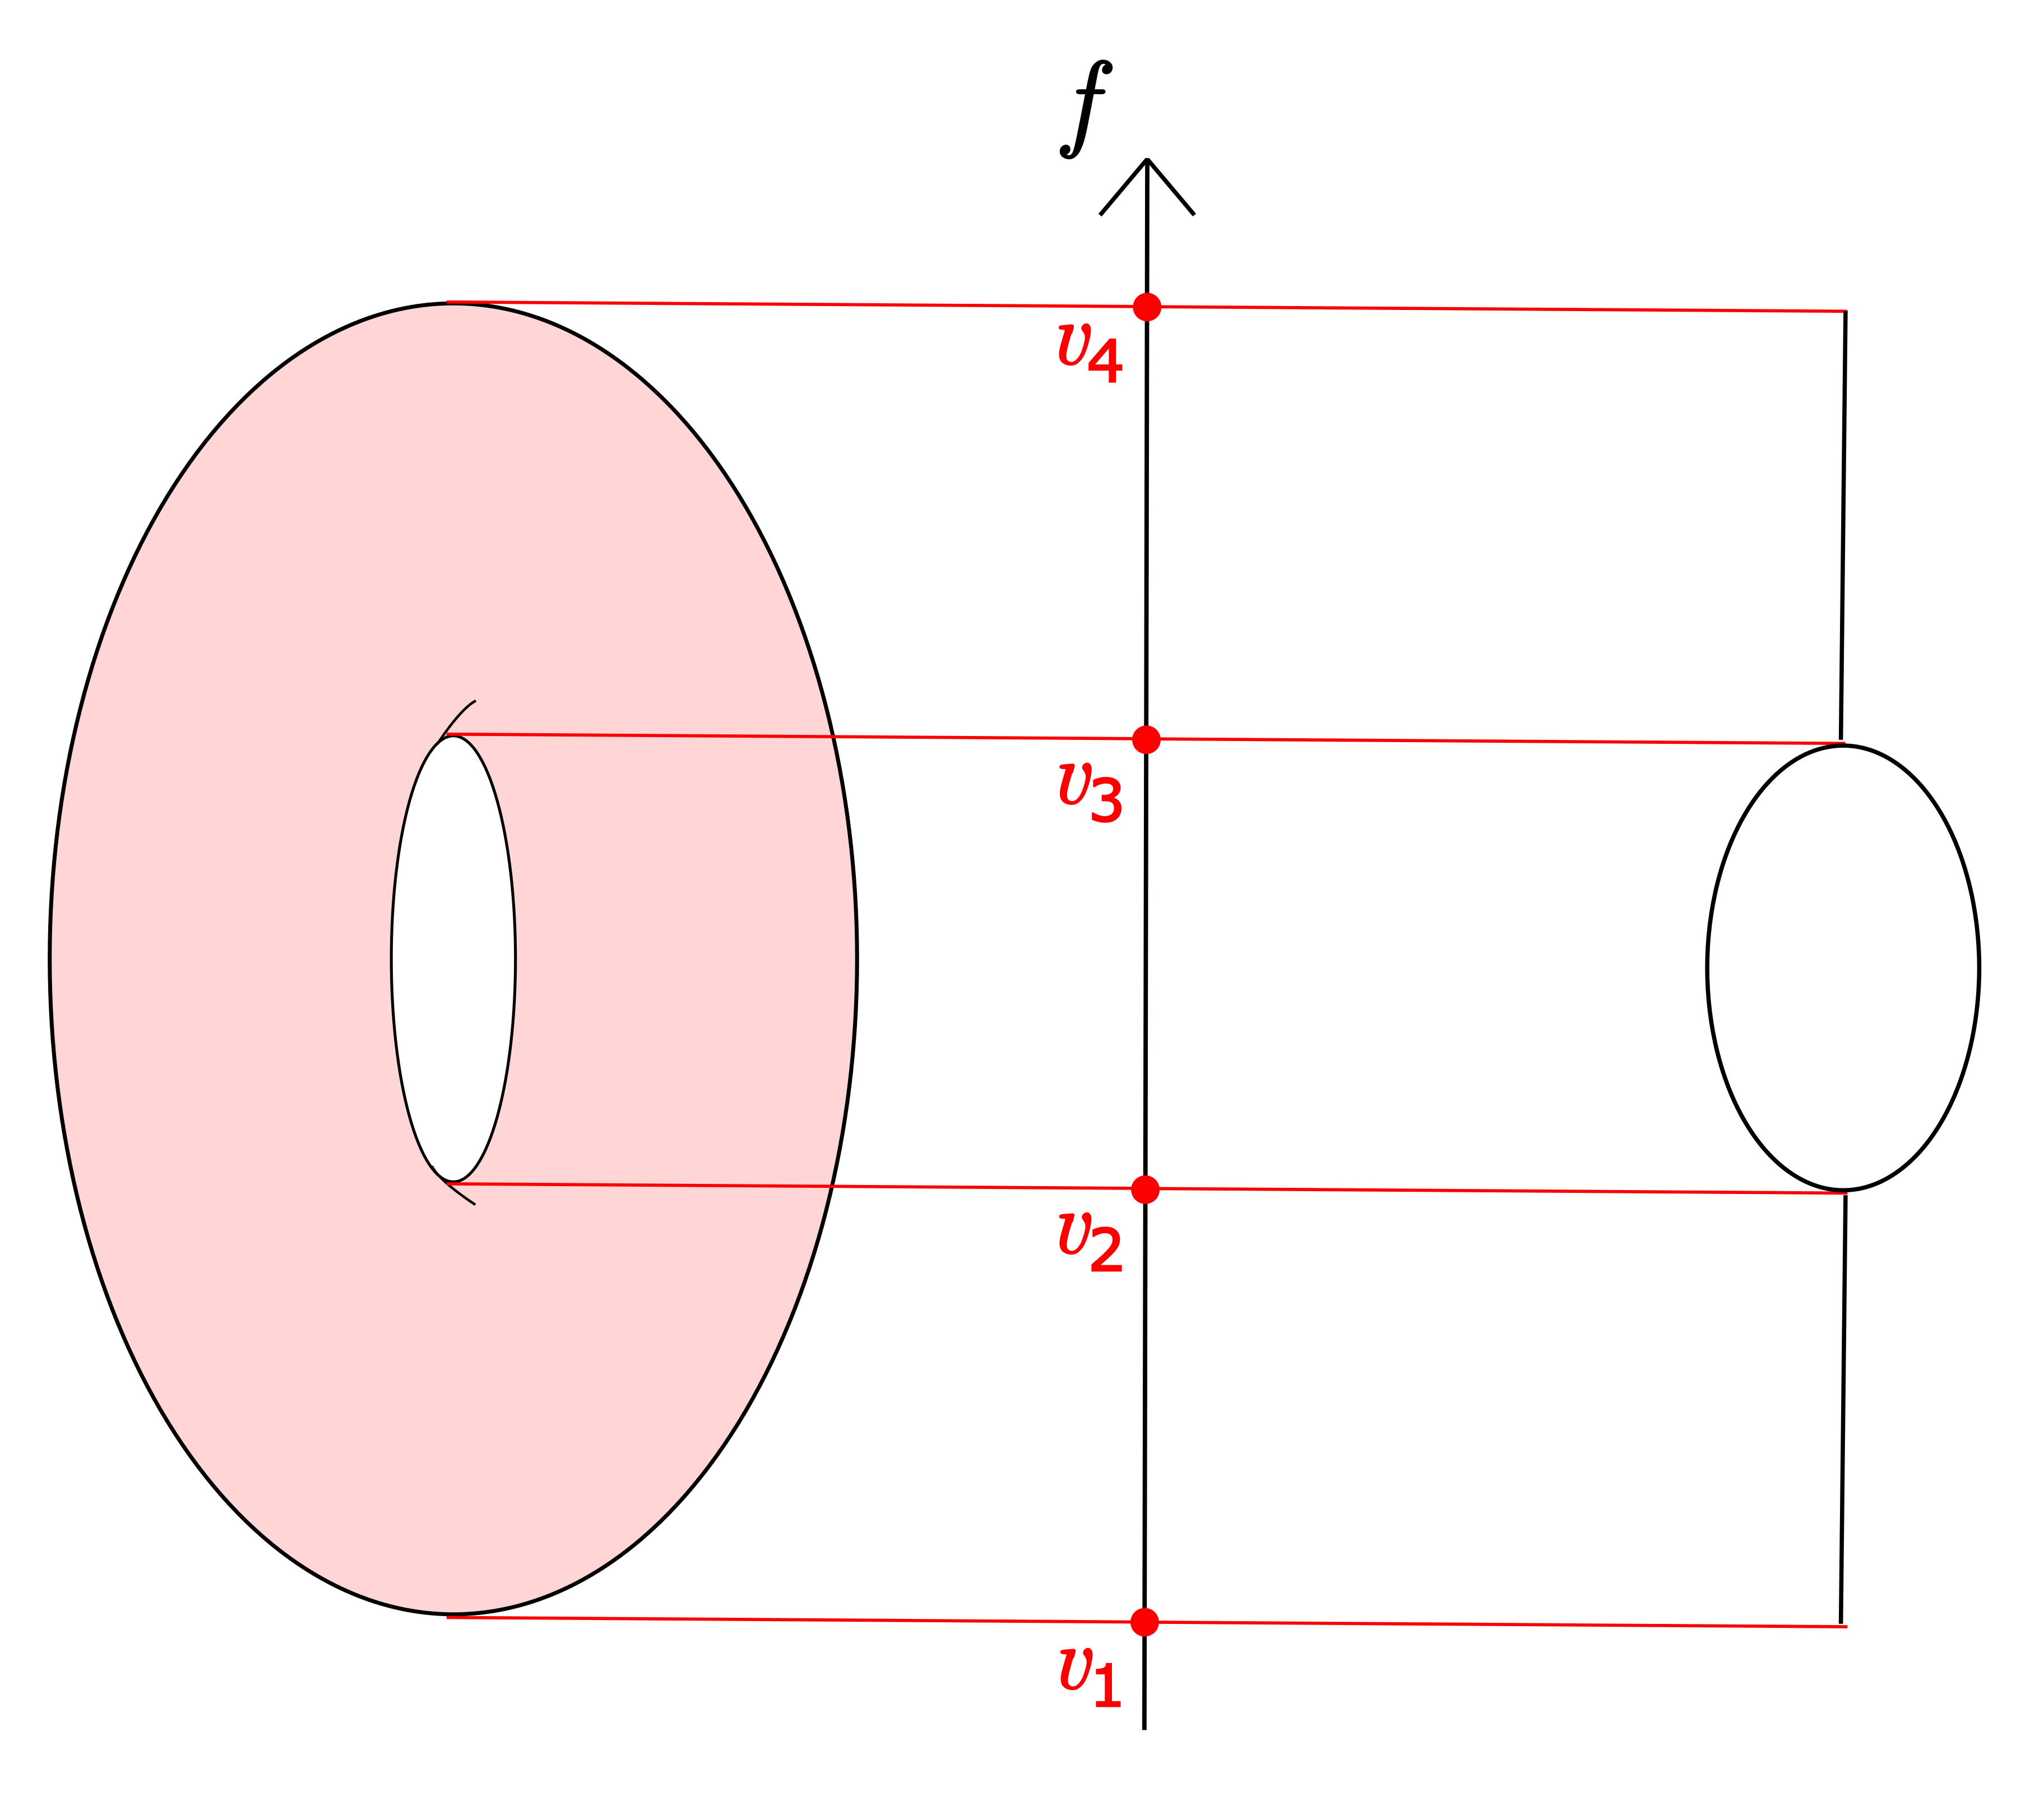
\includegraphics[width=0.5\textwidth]{images/reeb_graph.png}
    \caption{Example of a Reeb graph computed on a torus using height as filter function. The critical values $\{v_1,v_2,v_3,v_4\}$ of the filter function $f$ are represented in the middle. The Reeb graph is represented on the right.}
    \label{fig:reeb_graph_example}
\end{figure}


%\subsection{Mapper graphs}
Assume now that $(\spa,\dis)$ is  a metric space and let $f\colon\spa\rightarrow\R$ be a continuous function. The Mapper was introduced in \cite{singh2007topological} as a discrete and computable version of the Reeb graph $\Reeb_f(\spa)$. 
%in the sense  that it is a discrete and computable approximation of the Reeb graph computed with some filter function. 
%Indeed, it can be seen as a pixelized version of the Reeb graph. 
Assume that we are given a point cloud 
$\sample_n= \{x_1,\dots,x_n\}\subseteq \spa$ with known pairwise dissimilarities, as well as a filter function $f$ %is chosen and can be 
defined on each point of  $\sample_n$. The Mapper graph can then be computed with the following algorithm:
% on $\Xs_n$ computed with the filter function $f$ can be summarized as follows:
\begin{enumerate}
\item Cover the range of values $\Ys_n = f(\sample_n)$ with a set of consecutive intervals $\interv_1,\dots, \interv_r$  that overlap, i.e., one has $\interv_i\cap \interv_{i+1}\neq \varnothing$ for all $1\leq i \leq r-1$.
\item Group the points that fall in the same connected component of each preimage $\preim{f}{\interv_j}$, $j\in\{1,...,r\}$. This defines a {\it pullback cover}
$\mathcal{C}=\{\cluster_{1,1},\dots,\cluster_{1,k_1},\dots,\cluster_{r,1},\dots,\cluster_{r,k_r}\}$ of %the point cloud 
$\sample_n$. 
\item The Mapper graph is defined as the {\it nerve} of $\mathcal{C}$. Each node $v_{j,k}$ of the Mapper graph corresponds to an element $\cluster_{j,k}$ of $\mathcal C$, 
and two nodes $v_{j,k}$ and $v_{j',k'}$ are connected by an edge if and only if  $\cluster_{j,k} \cap \cluster_{j',k'} \neq \varnothing$.
\end{enumerate} 

Figure~\ref{fig:mapper_example} provides a Mapper graph computed on points sampled from a torus with its height as filter function, and a cover of the filter image with three intervals. 

\begin{figure}[t]
    \centering
    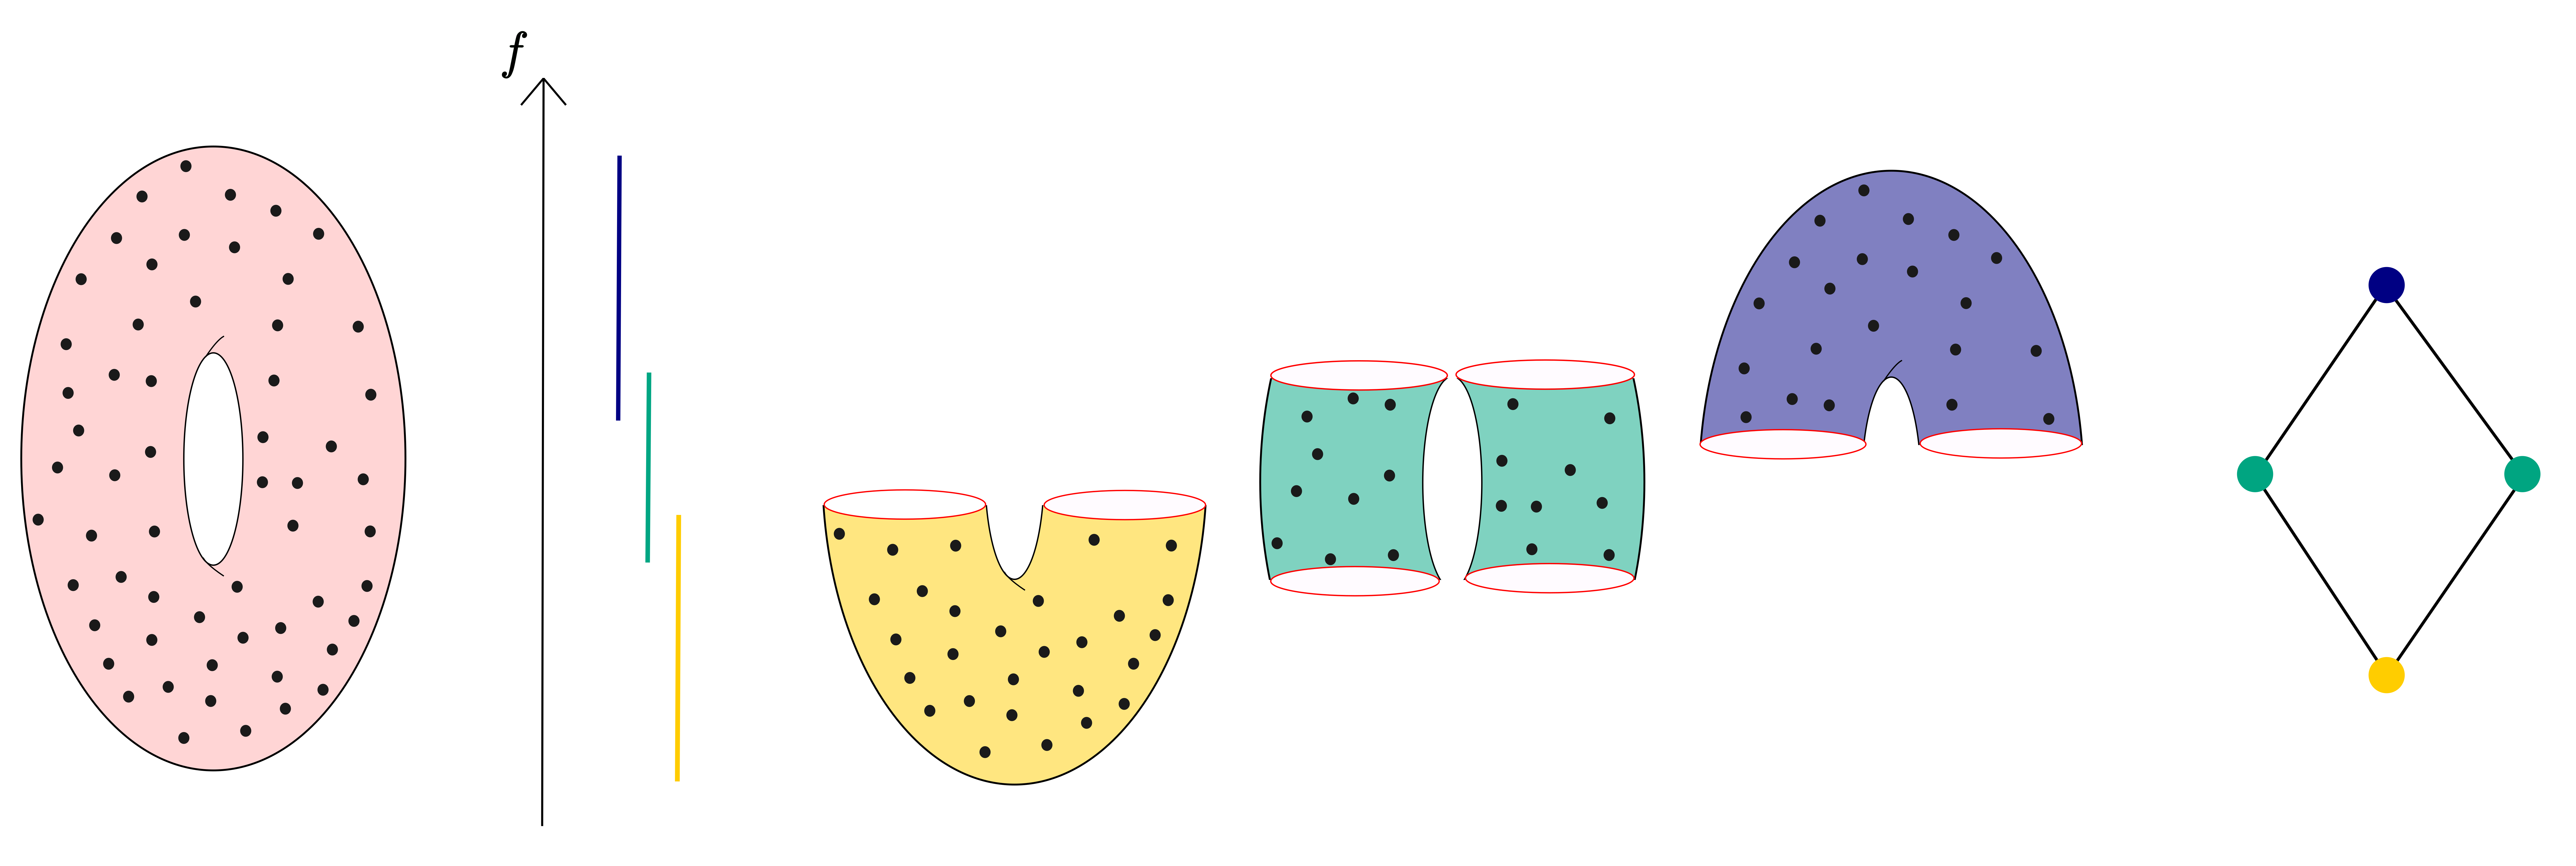
\includegraphics[width=\textwidth]{images/mapper.png}
    \caption{Example of a Mapper graph computed on points sampled from a torus with its height as filter function. The three intervals used for covering its image are represented in different colors.}
    \label{fig:mapper_example}
\end{figure}

In practice, the second step of the above algorithm is performed using a clustering algorithm, but we leave this consideration aside 
%adopt this general framework 
as it is more suitable for a theoretical discussion. Note that some clustering algorithms come with guarantees as to whether they are able to successfully estimate the connected components of the original space $\spa$. For example, in~\cite{niyogi2008finding}, Proposition~3.1. states that for points sampled from a Riemannian submanifold $\man$ of an Euclidean space, the union of Euclidean balls of radius $\eps$ centered on each sampled point for $\eps>0$ small enough has the same homology groups than $\man$, given that the sample is $\eps/2$ dense in $\man$ and under a geometric assumption on $\man$ (relating to its condition number). In particular, a clustering algorithm that consists in computing the connected components of an $\eps$-neighborhood graph of the sampled points will correctly estimate 
%where the points fall in 
the right connected components of $\man$. Spectral clustering also comes with strong guarantees, see for instance~\cite{arias2011spectral}.  


